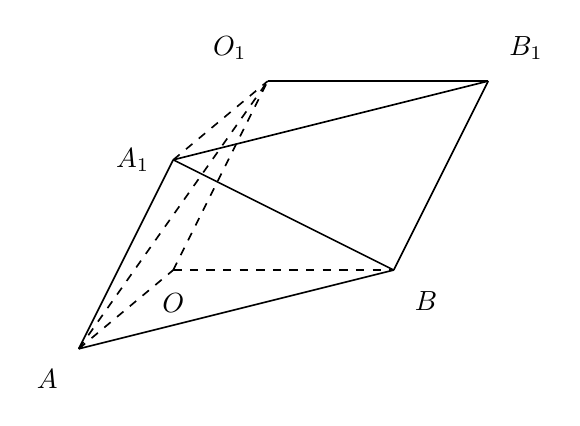
\begin{tikzpicture}[line width=.6pt, font=\normalsize]
\coordinate (A) at (0,0);
\coordinate (O) at (1.2,1.0);
\coordinate (B) at (4.0,1.0);
\coordinate (Oone) at (2.4000000000,3.4000000000);
\coordinate (Aone) at (1.2,2.4);
\coordinate (Bone) at (5.2000000000,3.4000000000);
% base triangle OAB
\draw[dashed] (A) -- (O);
\draw[dashed] (O) -- (B);
\draw (A) -- (B);
% top triangle O1A1B1
\draw (Bone) -- (Oone);
\draw (Aone) -- (Bone);
\draw[dashed] (Aone) -- (Oone);
% lateral edges
\draw (A) -- (Aone);
\draw[dashed] (O) -- (Oone);
\draw (B) -- (Bone);
% diagonals required by the problem: AO1 is A-A1 (solid) + A1-O1 (dashed)
\draw (Aone) -- (B);
\draw[dashed] (A)--(Oone);
% labels with clearance
\node[below left=4pt] at (A) {$A$};
\node[below=5pt] at (O) {$O$};
\node[below right=4pt] at (B) {$B$};
\node[above left=4pt] at (Oone) {$O_{1}$};
\node[left=5pt] at (Aone) {$A_{1}$};
\node[above right=4pt] at (Bone) {$B_{1}$};
\end{tikzpicture}
